\documentclass[12pt, a4paper]{report}
\usepackage[top=1.0in, bottom=1.0in, left=0.8in, right=0.8in]{geometry}

\setlength{\parskip}{\baselineskip}%
\setlength{\parindent}{0pt}%
\usepackage{bookmark}
\usepackage[]{graphicx}
\usepackage{enumitem}
\usepackage{amsmath}
\usepackage{relsize}
\usepackage{cprotect}
\usepackage{amsmath, amsfonts}
\usepackage{siunitx}
\usepackage{mathrsfs}
\usepackage{framed}
\usepackage{enumitem}
\usepackage{tikz}
\usepackage{circuitikz}
\usepackage{float}
\usepackage[english]{babel}
\usepackage{blindtext}

\newlist{notes}{enumerate}{1}
\setlist[notes]{label=\textbf{Note:} ,leftmargin=*}

\newlist{hints}{enumerate}{1}
\setlist[hints]{label=\textbf{Hint:} ,leftmargin=*}

\usepackage{xcolor}
\usepackage{color}
\definecolor{com1}{RGB}{125,125,125}
\definecolor{comment}{RGB}{140,115,115}
\definecolor{numbering}{rgb}{0.2,0.2,0.2}
\definecolor{key}{RGB}{0,0,180}
\definecolor{in}{RGB}{0,100,0}
\definecolor{out}{RGB}{100,30,30}
\definecolor{bg}{RGB}{245,245,245}
\definecolor{bgLight}{RGB}{250,250,250}
\definecolor{string}{RGB}{0,150,0}

\usepackage{hyperref}
\hypersetup{
    colorlinks=true,
    linkcolor=blue,
    filecolor=magenta,      
    urlcolor=blue,
}
\urlstyle{same}

\usepackage{listings}

\lstdefinestyle{py_code}{ %
    backgroundcolor=\color{bg},      % choose the background
    basicstyle=\ttfamily\small,		      % fonts
    breakatwhitespace=false,         % automatic breaks at whitespace ?
    breaklines=true,                 % sets automatic line breaking
    captionpos=b,                    % caption-position - bottom
    commentstyle=\itshape\color{comment},    % comment style
    extendedchars=true,              % use non-ASCII
    frame=single,	                   % single frame around the code
    keepspaces=true,                 % keeps spaces in text
    keywordstyle=\bfseries\color{key},% keyword style
    language=Python,                 	  % the language of the code
    morekeywords={Null},       % add more keywords to the set
    numbers=left,                    % line_numbers (none, left, right)
    numbersep=10pt,                  % line_no - code dist
    numberstyle=\footnotesize\color{numbering}, % line_no style
    rulecolor=\color{black},         % frame_color [!always set]
    showspaces=false,                % show spaces everywhere
    showstringspaces=false,          % 
    showtabs=false,                  % 
    stepnumber=1,                    % step b/w two line-no
    stringstyle=\color{string},     % string literal style
    tabsize=2,	                       % sets default tabsize to 2 spaces
    title=\lstname,                  % show the filename
    escapeinside={(*}{*)},			  % escape from style inside (* *)
    xleftmargin=\parindent,
    belowskip=-1.3 \baselineskip,
    aboveskip=1.0 \baselineskip,
    columns=fullflexible,
    xleftmargin=0.15in,
}
\lstnewenvironment{py_code}
{\lstset{style=py_code}}
{}

\lstdefinestyle{psudo}{ %
    backgroundcolor=\color{bgLight},   % choose the background
    basicstyle=\ttfamily\small,		      % fonts
    breakatwhitespace=false,         % automatic breaks at whitespace ?
    breaklines=true,                 % sets automatic line breaking
    captionpos=b,                    % caption-position - bottom
    commentstyle=\itshape\color{com1},          % comment style
    extendedchars=true,              % use non-ASCII
    keepspaces=true,                 % keeps spaces in text
    language=C,                 	  % the language of the code
    morekeywords={type,NULL, True, False},       % add more keywords to the set
    showspaces=false,                % show spaces everywhere
    showstringspaces=false,          % 
    showtabs=false,                  % 
    tabsize=2,	                       % sets default tabsize to 2 spaces
    title=\lstname,                  % show the filename
    escapeinside={(*}{*)},			  % escape from style inside (* *)
    belowskip=-1.8 \baselineskip,
    aboveskip=0.9 \baselineskip,
    columns=fullflexible,
    xleftmargin=0.2in,
    frame=tb,
    framexleftmargin=16pt,
    framextopmargin=6pt,
    framexbottommargin=6pt, 
    framerule=0pt,
}

\lstnewenvironment{psudo}
{\lstset{style=psudo}}
{}

\graphicspath{ ./ }


\title{\textbf{EE2703 : Applied Programming Lab \\ Assignment 3 \\ Fitting data to Models}} 
\author{Chagari Koushal Kumar Reddy \\ EE20B023} % Author name

\date{\today} % Date for the report

\begin{document}		
		
\maketitle % Insert the title, author and date
\section*{Aim}
The aim of this assignment is to :
\begin{itemize}
    \item Record data from a noisy environment and process it
    \item Fit the data using a given model
    \item Observe how fitting model paramters vary with noise
\end{itemize}

\section*{Theory}
Run the python file "generate\_data.py" to generate the file 
"fitting.dat" which has 10 columns, the first one being time and the rest being different amounts of noise added to the function. 
The data columns correspond to the following equation:

    \begin{equation}\label{eq:1}
    f(t) = 1.05J_{2}(t)-0.105t+n(t)
    \end{equation}

Here $n(t)$ is the noise added which
follows normal distribution given by:\\
    \begin{equation*}
        Pr(n(t)|\sigma) = \frac{1}{\sigma \sqrt{2 \pi}} \exp(- \frac{n(t)^2}{2 \sigma ^2})
    \end{equation*}

where $\sigma$ is generated using the python function "logspace"
 
    \begin{psudo}
    sigma = logspace(-1,-3,9)\end{psudo}
 
The model function which is used to fit the data is:
    \begin{equation}\label{eq2}
        g(t;A,B) = AJ_{2}(t) + Bt
    \end{equation}
with true values of A, B being
    \begin{equation*}
        A = 1.05,  B = -0.105
    \end{equation*}

To solve this problem, we first create the matrix M whose second column is
the time vector and the corresponding values of the Bessel function
$J_{2}(t)$ is the first column. Another column vector $p$ is created where
the first element is $A$ and second element is $B$. We obtain $g(t;A,B)$ as a column vector
by multiplying matrices M and p.

    \begin{equation}\label{eq3}
        g(t;A,B) = \begin{pmatrix}
            J_{2}(t_{1}) & t_{1}\\
            \ldots      &  \ldots\\
            J_{2}(t_{m}) & t_{m}
        \end{pmatrix}
        .
        \begin{pmatrix}
            A\\B
        \end{pmatrix}
        = M.p
    \end{equation}

Now the mean square error for the data is found for $A=0,0.1,\ldots\ ,2$
and $B=-0.2,-0.19,\ldots\ ,0$ using the formula

\begin{equation}\label{eq4}
    \epsilon _{ij} = \frac{1}{101} \sum\limits_{k=0}^{101} (f_{k}-g(t;A,B))^{2}
\end{equation}

where $f_{k}$ is the first column of data. A contour plot of the mean square error
with the values of $A$ and $B$ gives an idea of how error varies with $A$, $B$.
 By analyzing the graph we can find for which values of $A$, $B$ minimum error occurs.

An estimate of the values of $A$ and $B$ to fit the given noisy data is found using the
method of least squares. The required python command is
\begin{psudo}
    scipy.linalg.lstsq(M,Data_column_to_be_fitted)
\end{psudo}

The above command gives an estimate for $A$ and $B$ which minimizes the mean square error.
\section*{Codes}
The Python function used to compute $g(t;A,B)=AJ_{2}(t)+Bt$ is as follows:

\begin{py_code}
    def g(t,A,B):
        j2_t = sp.jv(2,t)
        return A*j2_t + B*t
\end{py_code}

The piece of python code used to calculate the mean square error
for $A=0,0.1,\ldots\ ,2$ and $B=-0.2,-0.19,\ldots\ ,0$ is as follows:

\begin{py_code}
    a = np.linspace(0, 2, 21)
    b = np.linspace(-0.2, 0, 21)
    MSE = np.zeros((len(a), len(b)))
    
    for i in range(len(a)):
        for j in range(len(b)):
            diff = np.zeros(0)      # Empty array
            for k in range(0, len(time)):
                g_value = np.array([g(t, a[i], b[j]) for t in time])
                diff = np.append(diff, (f_with_noise[0][k] - g_value[k])**2)     # f_with_noise[0][k] is the first column of data
            MSE[i][j] = diff.mean()
\end{py_code}

\section*{Results and Plots}
\begin{enumerate}
    \item The noisy datasets from "fitting.dat" are plotted here. The first column of "fitting.dat" corresponds to time and the remaining 9 columns
correspond to the function with noise.
    \begin{figure}[H]
        \centering
        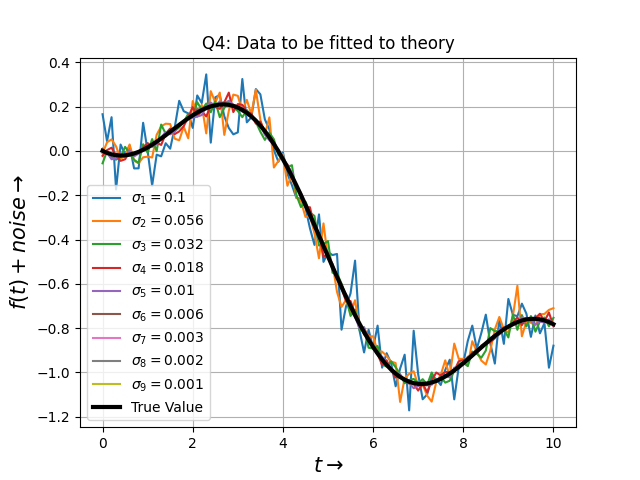
\includegraphics[scale = 0.76]{Figure_0.png}
        \caption{Data Plot}
        \label{fig:sample}
    \end{figure}

    \item Error bars are used to show the deviation of noisy data(Here of first column)
from the true value. The bright red dot in the center is the value of first column.
    \begin{figure}[H]
        \centering
        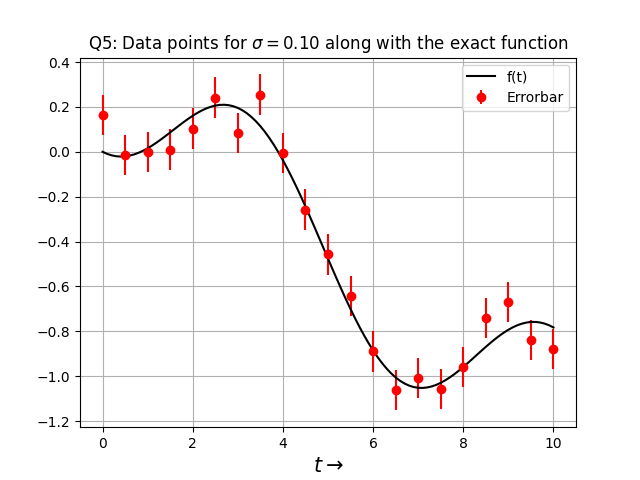
\includegraphics[scale = 0.735]{Figure_1.png}
        \caption{Error Bars}
        \label{fig:sample}
    \end{figure}

    \item Contour plots of Mean squared error are plotted for various values of $A$ and $B$.
    \begin{figure}[H]
        \centering
        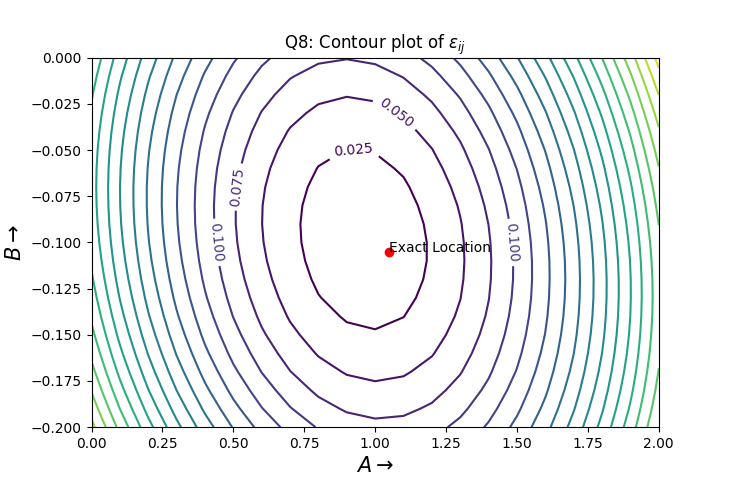
\includegraphics[scale = 0.8]{Figure_2.png}
        \caption{Contour Plot}
        \label{fig:sample}
    \end{figure}

    \item This is the plot of deviation of parameters $A$, $B$ from their true
values with respect to the standard deviation of the noise present in the data (Linear scale).
    \begin{figure}[H]
        \centering
        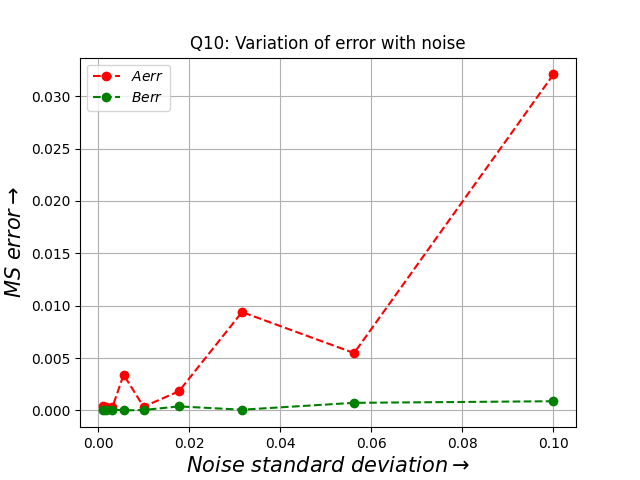
\includegraphics[scale = 0.8]{Figure_3.png}
        \caption{Linear scale Error plot}
        \label{fig:sample}
    \end{figure}

    \item This is the plot of deviation of parameters $A$, $B$ from their true
    values with respect to the standard deviation of the noise present in the data (Logarithmic scale).
    \begin{figure}[H]
        \centering
        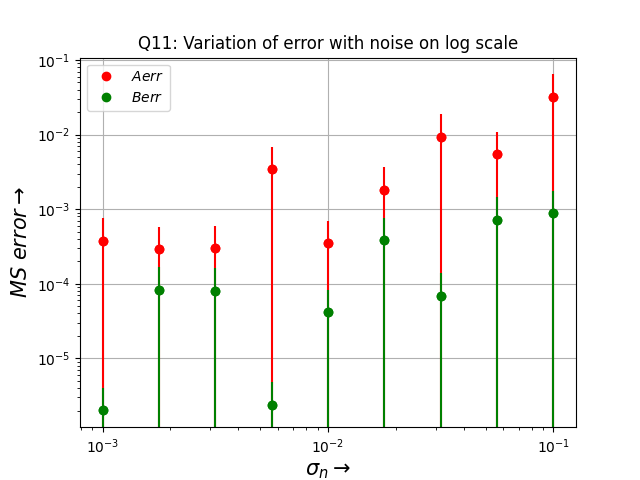
\includegraphics[scale = 0.8]{Figure_4.png}
        \caption{Logarithmic scale Error plot}
        \label{fig:sample}
    \end{figure}
    The logarithmic errors of $A$, $B$ show somewhat linear behaviour with few deviations.    
\end{enumerate}

\section*{Observations and Conclusions}
   \begin{itemize}
    \item From the error bar plot we observe the estimated parameters of $A$, $B$ provide a very close fit to the
actual values of the function with noise of standard deviation $0.1$.
  	\item From the contour plot it is observed that the mean squared error converges to a minimum value
as $A$, $B$ approach their true values which are 1.05, -0.105 respectively. For the noisy data there is a single 
minima which is obtained using the least square solution.
  	\item The errors in the estimate of $A$, $B$ are not varying in a linear fashion
with respect to time. Also the error in $A$ is more suspectible to noise than $B$. This implies that
the Bessel's function values accounts more to the noise than the time values.
    \item Logarithmic errors of $A$, $B$ are linearly varying with respect to the logarithm of noise
with slight deviations. This linear relation means that the errors in estimate of $A$, $B$ vary exponentially with
standard deviation of noise as seen in Figure 4. 
  \end{itemize}

\end{document}